\documentclass[a4paper,12px]{article}

\usepackage{graphicx}
\usepackage[english]{babel}
\usepackage{fancyhdr}
\usepackage{lastpage}
\usepackage{xifthen}
\usepackage[linesnumberedhidden, titlenotnumbered]{algorithm2e}
\usepackage{lipsum}
\usepackage{hyperref}
\usepackage{array}
\usepackage{tabularx}

\usepackage{minted}
\usepackage{caption}
\usepackage{amssymb}

\pagestyle{fancy}
\lhead{
\includegraphics[width=7cm]{logoUvA}}
\rhead{\footnotesize \textsc {Report\\ \opdracht}}
\lfoot
{%
    \footnotesize \studentA
    \ifthenelse{\isundefined{\studentB}}{}{\\ \studentB}
    \ifthenelse{\isundefined{\studentC}}{}{\\ \studentC}
    \ifthenelse{\isundefined{\studentD}}{}{\\ \studentD}
    \ifthenelse{\isundefined{\studentE}}{}{\\ \studentE}
}
\cfoot{}
\rfoot{\small \textsc {Page \thepage\ of \pageref{LastPage}}}
\renewcommand{\footrulewidth}{0.5pt}

\fancypagestyle{firststyle}
{%
    \fancyhf{}
    \renewcommand{\headrulewidth}{0pt}
    \chead{
\includegraphics[width=7cm]{logoUvA}}
    \rfoot{\small \textsc {Page \thepage\ of \pageref{LastPage}}}
}

\setlength{\topmargin}{-0.3in}
\setlength{\textheight}{630pt}
\setlength{\headsep}{40pt}

% =================================== DOC INFO ===================================

\newcommand{\titel}{Gradients and Slope fields}
\newcommand{\opdracht}{Python Assignment 2}
\newcommand{\docent}{Dr. A.J.P. Heck}
\newcommand{\cursus}{Numerical Recipes Project}
\newcommand{\vakcode}{5062NURP6Y}
\newcommand{\datum}{\today}
\newcommand{\studentA}{Robin Klusman}
\newcommand{\uvanetidA}{10675671}
\newcommand{\studentB}{Maico Timmerman}
\newcommand{\uvanetidB}{10542590}
%\newcommand{\studentC}{Boudewijn Braams}
\newcommand{\uvanetidC}{10401040}
%\newcommand{\studentD}{Govert Verkes}
\newcommand{\uvanetidD}{10211748}
%\newcommand{\studentE}{Naam student 5}
\newcommand{\uvanetidE}{UvAnetID student 5}

% ===================================  ===================================

\begin{document}
\thispagestyle{firststyle}
\begin{center}
    \textsc{\Large \opdracht}\\[0.2cm]
    \rule{\linewidth}{0.5pt} \\[0.4cm]
    {\huge \bfseries \titel}
    \rule{\linewidth}{0.5pt} \\[0.2cm]
    {\large \datum  \\[0.4cm]}
    \begin{minipage}{0.4\textwidth}
        \begin{flushleft}
            \emph{Student:}\\
            {\studentA \\ {\small \uvanetidA \\[0.2cm]}}
            \ifthenelse{\isundefined{\studentB}}{}{\studentB \\ {\small \uvanetidB \\[0.2cm]}}
            \ifthenelse{\isundefined{\studentC}}{}{\studentC \\ {\small \uvanetidC \\[0.2cm]}}
            \ifthenelse{\isundefined{\studentD}}{}{\studentD \\ {\small \uvanetidD \\[0.2cm]}}
            \ifthenelse{\isundefined{\studentE}}{}{\studentE \\ {\small \uvanetidE \\ [0.2cm]}}
        \end{flushleft}
    \end{minipage}~%
    \begin{minipage}{0.4\textwidth}
        \begin{flushright}
            \emph{Supervisor:} \\
            \docent \\[0.2cm]
            \emph{Course:} \\
            \cursus \\[0.2cm]
            \emph{Course code:} \\
            \vakcode \\[0.2cm]
        \end{flushright}
    \end{minipage}\\[1 cm]
\end{center}


% =================================== FRONT PAGE ===================================

\vspace{2cm}
\begin{center}
    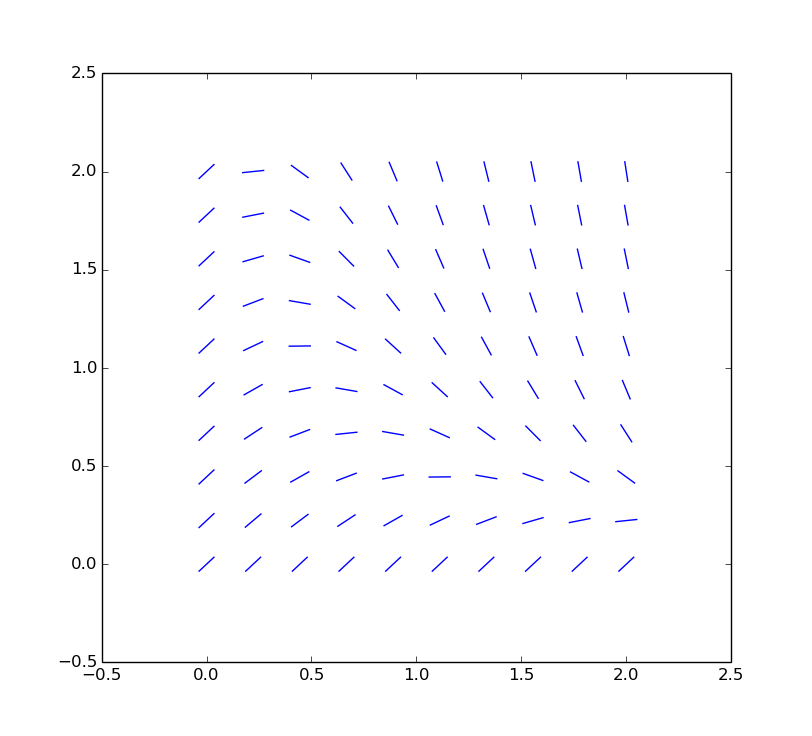
\includegraphics[width=(\textwidth/6*5)]{slopefield}
\end{center}
\clearpage

\tableofcontents
\vspace{5mm}

\captionsetup{width=\textwidth/7*5}

% =================================== MAIN TEXT ===================================

\section{Gradients}
\subsection{Gradient Arrows}



\begin{center}
    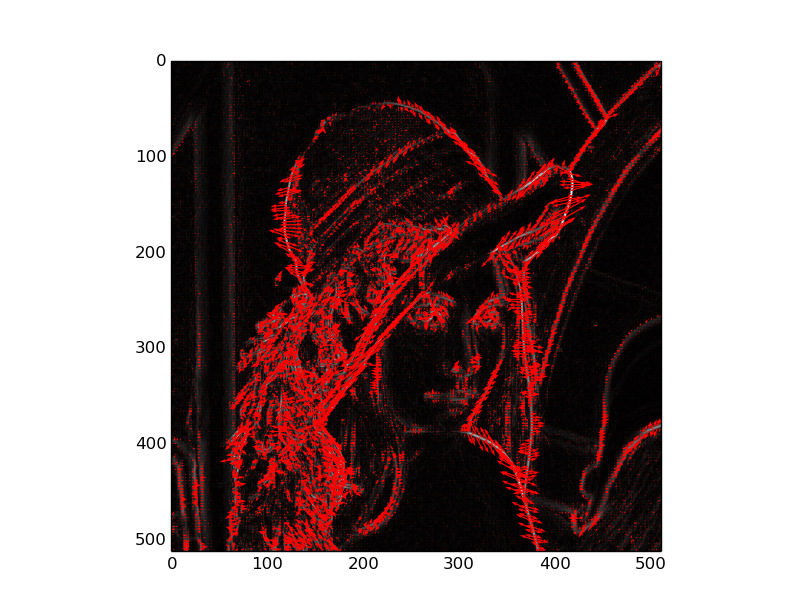
\includegraphics[width=\textwidth]{gradient}
    \captionof{figure}{}
\end{center}

\subsection{Gaussian blur}



\begin{center}
    
\includegraphics[width=\textwidth]{gauss}
    \captionof{figure}{}
\end{center}

\subsection{Laplace operator}



\begin{center}
    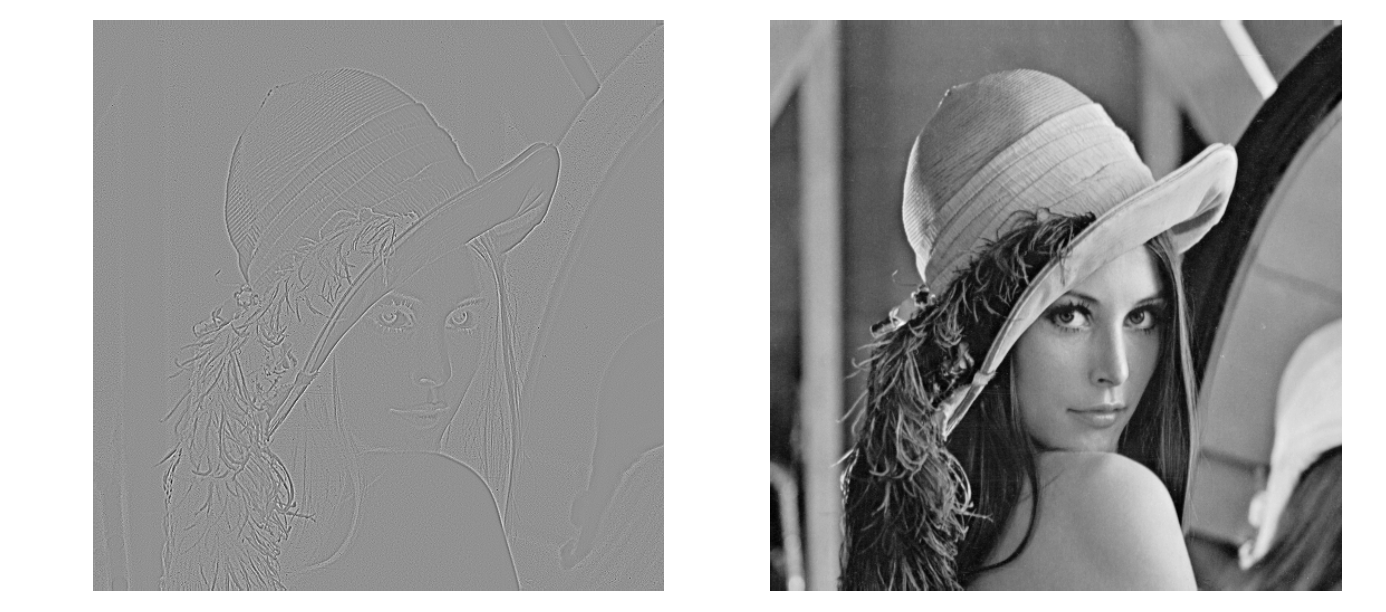
\includegraphics[width=\textwidth]{laplace}
    \captionof{figure}{}
\end{center}

\subsection{Sobel operator}



\begin{center}
    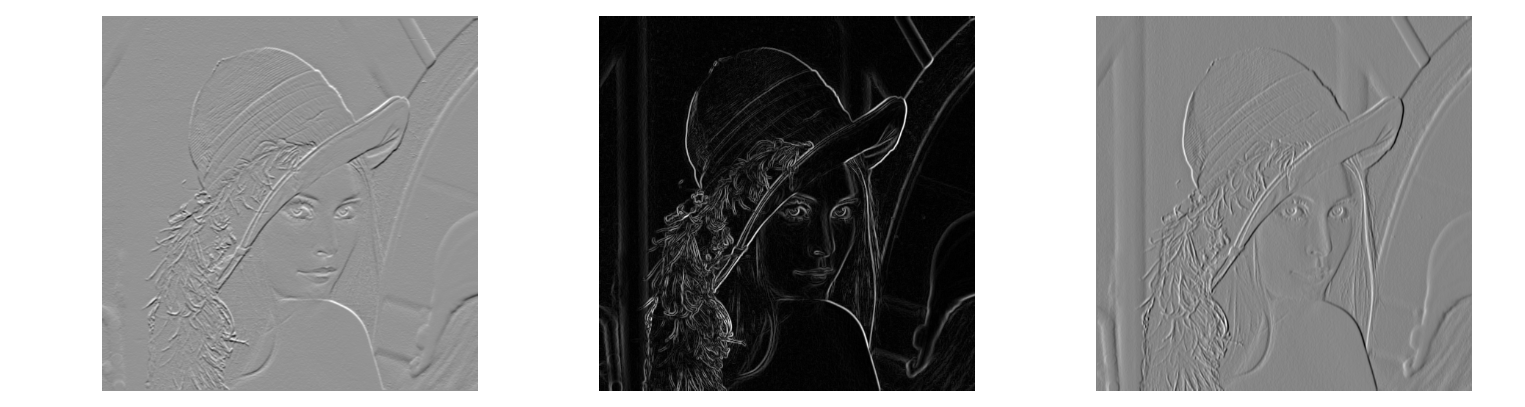
\includegraphics[width=\textwidth]{sobel}
    \captionof{figure}{}
\end{center}

\clearpage
\section{Slope Fields}
\subsection{Slope and random fields}

In this exercise first a slope field of equally spaced slope lines is created,
after which a slope field of 2000 randomly positioned slope lines is created.
For both of these slope fields, the first problem was to make lines of equal
length at an angle corresponding to the slope of the function in the point
$(a,b)$ with $(a,b)$ at its center. To create these lines the $\Delta t$ and
$\Delta y$ from $(a,b)$ has to be calculated. We can then draw a line from
$(a-\Delta t, b-\Delta y)$ to $(a+\Delta t, b+\Delta y)$ to get our line.

Calculating $\Delta t$ and $\Delta y$ required a combination of goniometric
formulas to find $\Delta y$ and the Pythagoras theorem to find $\Delta t$.  We
used $\Delta y = c*\sin(\tan^{-1}(s))$ where $c$ is half the total
desired line length and $s$ is the slope. Then $\Delta t$ is found by simply
$\Delta t= \sqrt{c^2-\Delta y^2}$

In case of the structured slope field we plotted a total of 100 slope lines on
the interval $(0,2)$ in both the $t$ and $y$ directions as shown in the image
below.
\begin{center}
    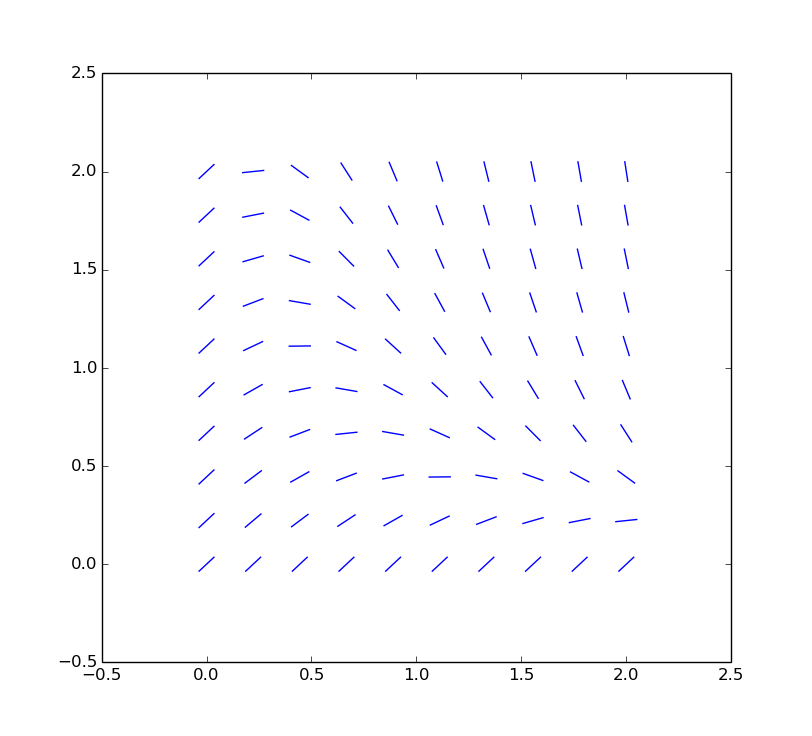
\includegraphics[width=\textwidth]{slopefield}
    \captionof{figure}{Structured slope field for $\varphi(t,y) = 1-2ty$ with a
        total of 100 slope lines.}
\end{center}

For the random slope field two random numbers are generated, one for the
$t$-coordinate and one for the $y$-coordinate. This is repeated a total of 2000
times to create the field as shown in the image below.
\begin{center}
    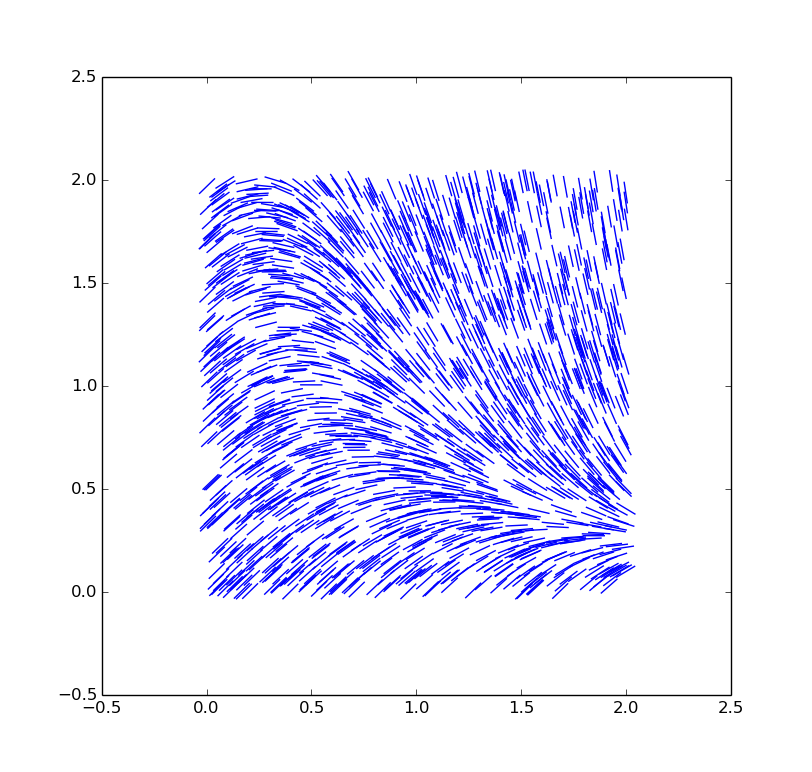
\includegraphics[width=\textwidth]{randomfield}
    \captionof{figure}{Random slope field for $\varphi(t,y) = 1-2ty$ with a
        total of 2000 slope lines.}
\end{center}

\subsection{Euler approximation}

For the Euler approximation a program had to be written that approximates the
graph of a function using the Euler method. This method does a certain amount of
steps over a certain interval and each time calculates how much has to be added
to the value of the previous step to get the value for this step.
$y_{k+1}=y_k+h*\varphi (t_k,y_k)$ where $y_k$ is the function value of the
previous step, $h$ is the step width and $t_k$ is the $t$ value of the  this
step. After calculating the new $y$ value the new $t$ value is produced by
$t_{k+1} = t_k + h$.

When repeating this process 2000 times on the interval $(0,2)$ for $\varphi(t,
y) = 1-2ty$ with begin values $y(0) = 1.5$ and $y(0) = 0.25$ it creates the
function approximation shown in the figure below.

\begin{center}
    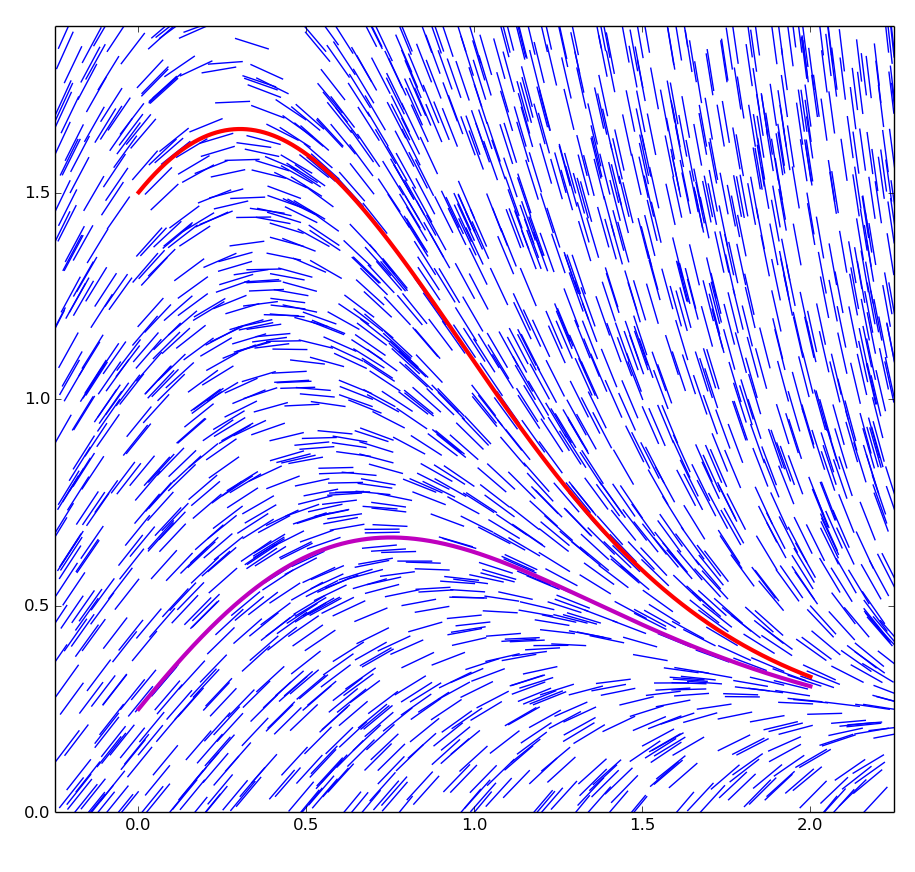
\includegraphics[width=\textwidth]{euler1}
    \captionof{figure}{Shows a random slope field of $\varphi(t,y)=1-2ty$ with
        the corresponding Euler approximation of the graph. Using $y(0) = 1.5$
        in red and $y(0) = 0.25$ in purple.}
\end{center}

In the case of $\varphi(t,y)=y(1-1/3y)$ on the interval $(-1, 1)$ with begin
values $y(-1)=0.25$ in red and $y(-1) = 2.5$ in purple.

\begin{center}
    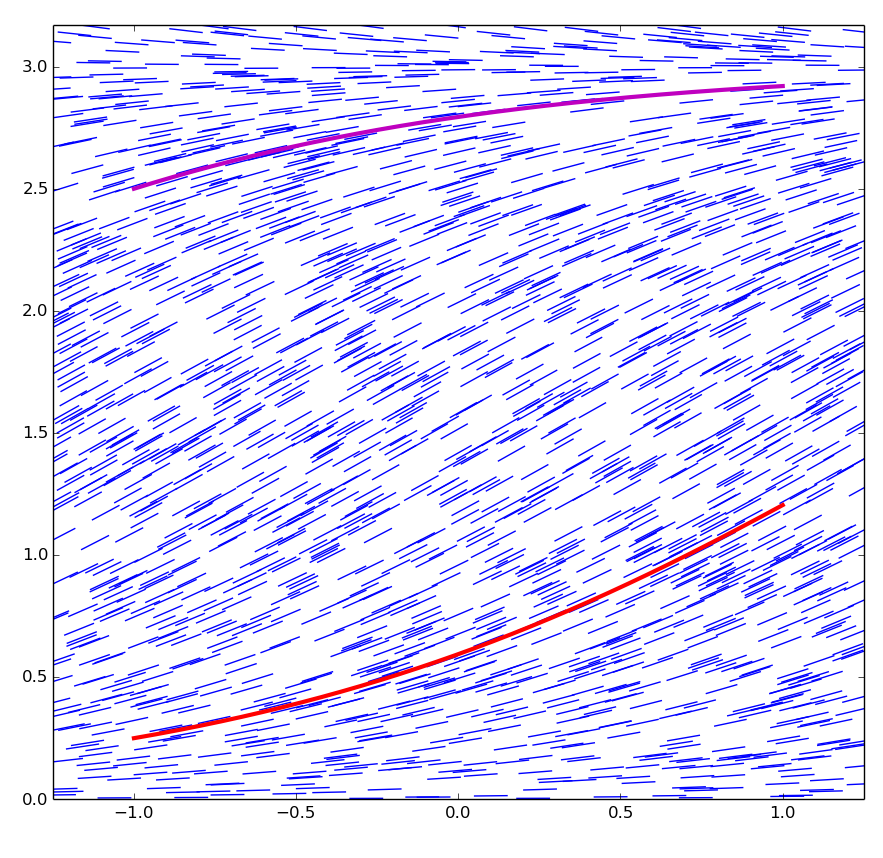
\includegraphics[width=\textwidth]{euler2}
    \captionof{figure}{Shows a random slope field of $\varphi(t,y)=y(1-1/3y)$ with
        the corresponding Euler approximation of the graph. Using $y(-1) = 0.25$
        in red and $y(-1) = 2.5$ in purple.}
\end{center}


% =================================== REFERENCES ===================================

%\clearpage
%\bibliographystyle{unsrt}
%\bibliography{bib}

\end{document}
